\documentclass{article}
\usepackage{graphicx} % Required for inserting images
\usepackage{float}

\title{2D Gray-Scott Model}
\author{Skupina 16: Luka Pantar, Mark Loboda}
\date{April 2025}

\begin{document}

\maketitle

\section{Introduction}
\subsection{Serial}
This algorithm performs a reaction-diffusion system called the \textit{Gray-Scott model} that simulates the behavior of two species over time and space in two dimensions. Interesting patterns emerge from the simulation over time. This algorithm runs on one thread without any parallelization.

\subsection{Parallel}
This algorithm performs the same simulation but is only parallelized using \textit{CUDA} to run on the GPU. We parallelized computation of each cell in the grid and ran a kernel for each step of the simulation. Between kernel runs, the device grid pointers are swapped around to not require any copies between steps. 

\subsection{Parallel Optimized}
\label{sub13:parallel_optimized}
This algorithm takes the basic parallel algorithm and further optimizes its execution with different approaches. The main optimization we made to the algorithm was the use of shared memory for each block of threads and the utilization of two GPUs to compute the steps of the algorithm. We further optimized our solution with the following changes:
\begin{enumerate}
    \item We used caching of values to minimize the number of times the algorithm needed to access the grid data in memory, which gained us a bit of performance, as the calculations had to access the array a couple of times per cell.
    \item We used \texttt{float2} instead of two \texttt{float}s in our struct, which represents a single cell and contains two values, U and V, which gained quite a lot of performance due to faster loading and access of a single 64-bit value compared to two 32-bit values.
    \item We removed pointer-of-pointer access used in other algorithms for convenience and replaced it with a flattened array.
    \item We switched the expansive modulus operator for wrap-around with a single, cheaper conditional statement. 
\end{enumerate}

\section{Results}
We ran a benchmark of our algorithms where we ran each algorithm eight times for five different grid sizes. We discarded the worst run of each algorithm as the execution times were significantly larger because of kernel caching on the GPU. Then we also discarded three of the worst times, as the times in some cases are too low to run consistently and sometimes resulted in much higher times, which could’ve been for other reasons and not the algorithm implementation itself.

The figure~\ref{fig:avg_times} shows that the execution times of the serial implementation are significantly slower even on smaller grid sizes and only get worse as the grid size increases. A simple parallelization improves on the serial algorithm by the orders of 100 in terms of speedup, as shown in Figure 2~\ref{fig:speedups}. As the grid size increases, the difference becomes even more apparent.

The parallel optimized algorithm, run on one GPU, optimizes the basic parallel implementation and is described in section~\ref{sub13:parallel_optimized}. We can see a constant improvement when compared to the basic parallel algorithm on all grid sizes in figure~\ref{fig:speedups}. 

The last algorithm runs the same procedure as the optimized parallel algorithm, only splitting the grid into two equally sized grids and running them independently on two GPUs. The execution times of this algorithm are much worse on all grid sizes we tested. We can observe a much better comparison of the two algorithms as the grid size increases and predict that for even larger grids, the two GPU implementation would perform better.

\begin{table}[H]
    \centering
    \begin{tabular}{| l || c | c | c | c | c |}
        \hline
        Algorithm & 256x256 & 512x512 & 1024x1024 & 2048x2048 & 4096x4096 \\
        \hline
        Serial & 4727 & 13883 & 50175 & 193547 & 764905 \\
        Parallel & 33 & 42 & 141 & 488 & 1984 \\
        Parallel Optimized (1 GPU) & 26 & 33 & 117 & 401 & 1531 \\
        Parallel Optimized (2 GPUs) & 610 & 621 & 671 & 875 & 1565 \\
        \hline
    \end{tabular}
    \caption{Average total time per grid size for each algorithm, measured in \textbf{milliseconds [ms]}.}
    \label{tbl:avg_times}
\end{table}

\begin{figure}[H]
    \centering
    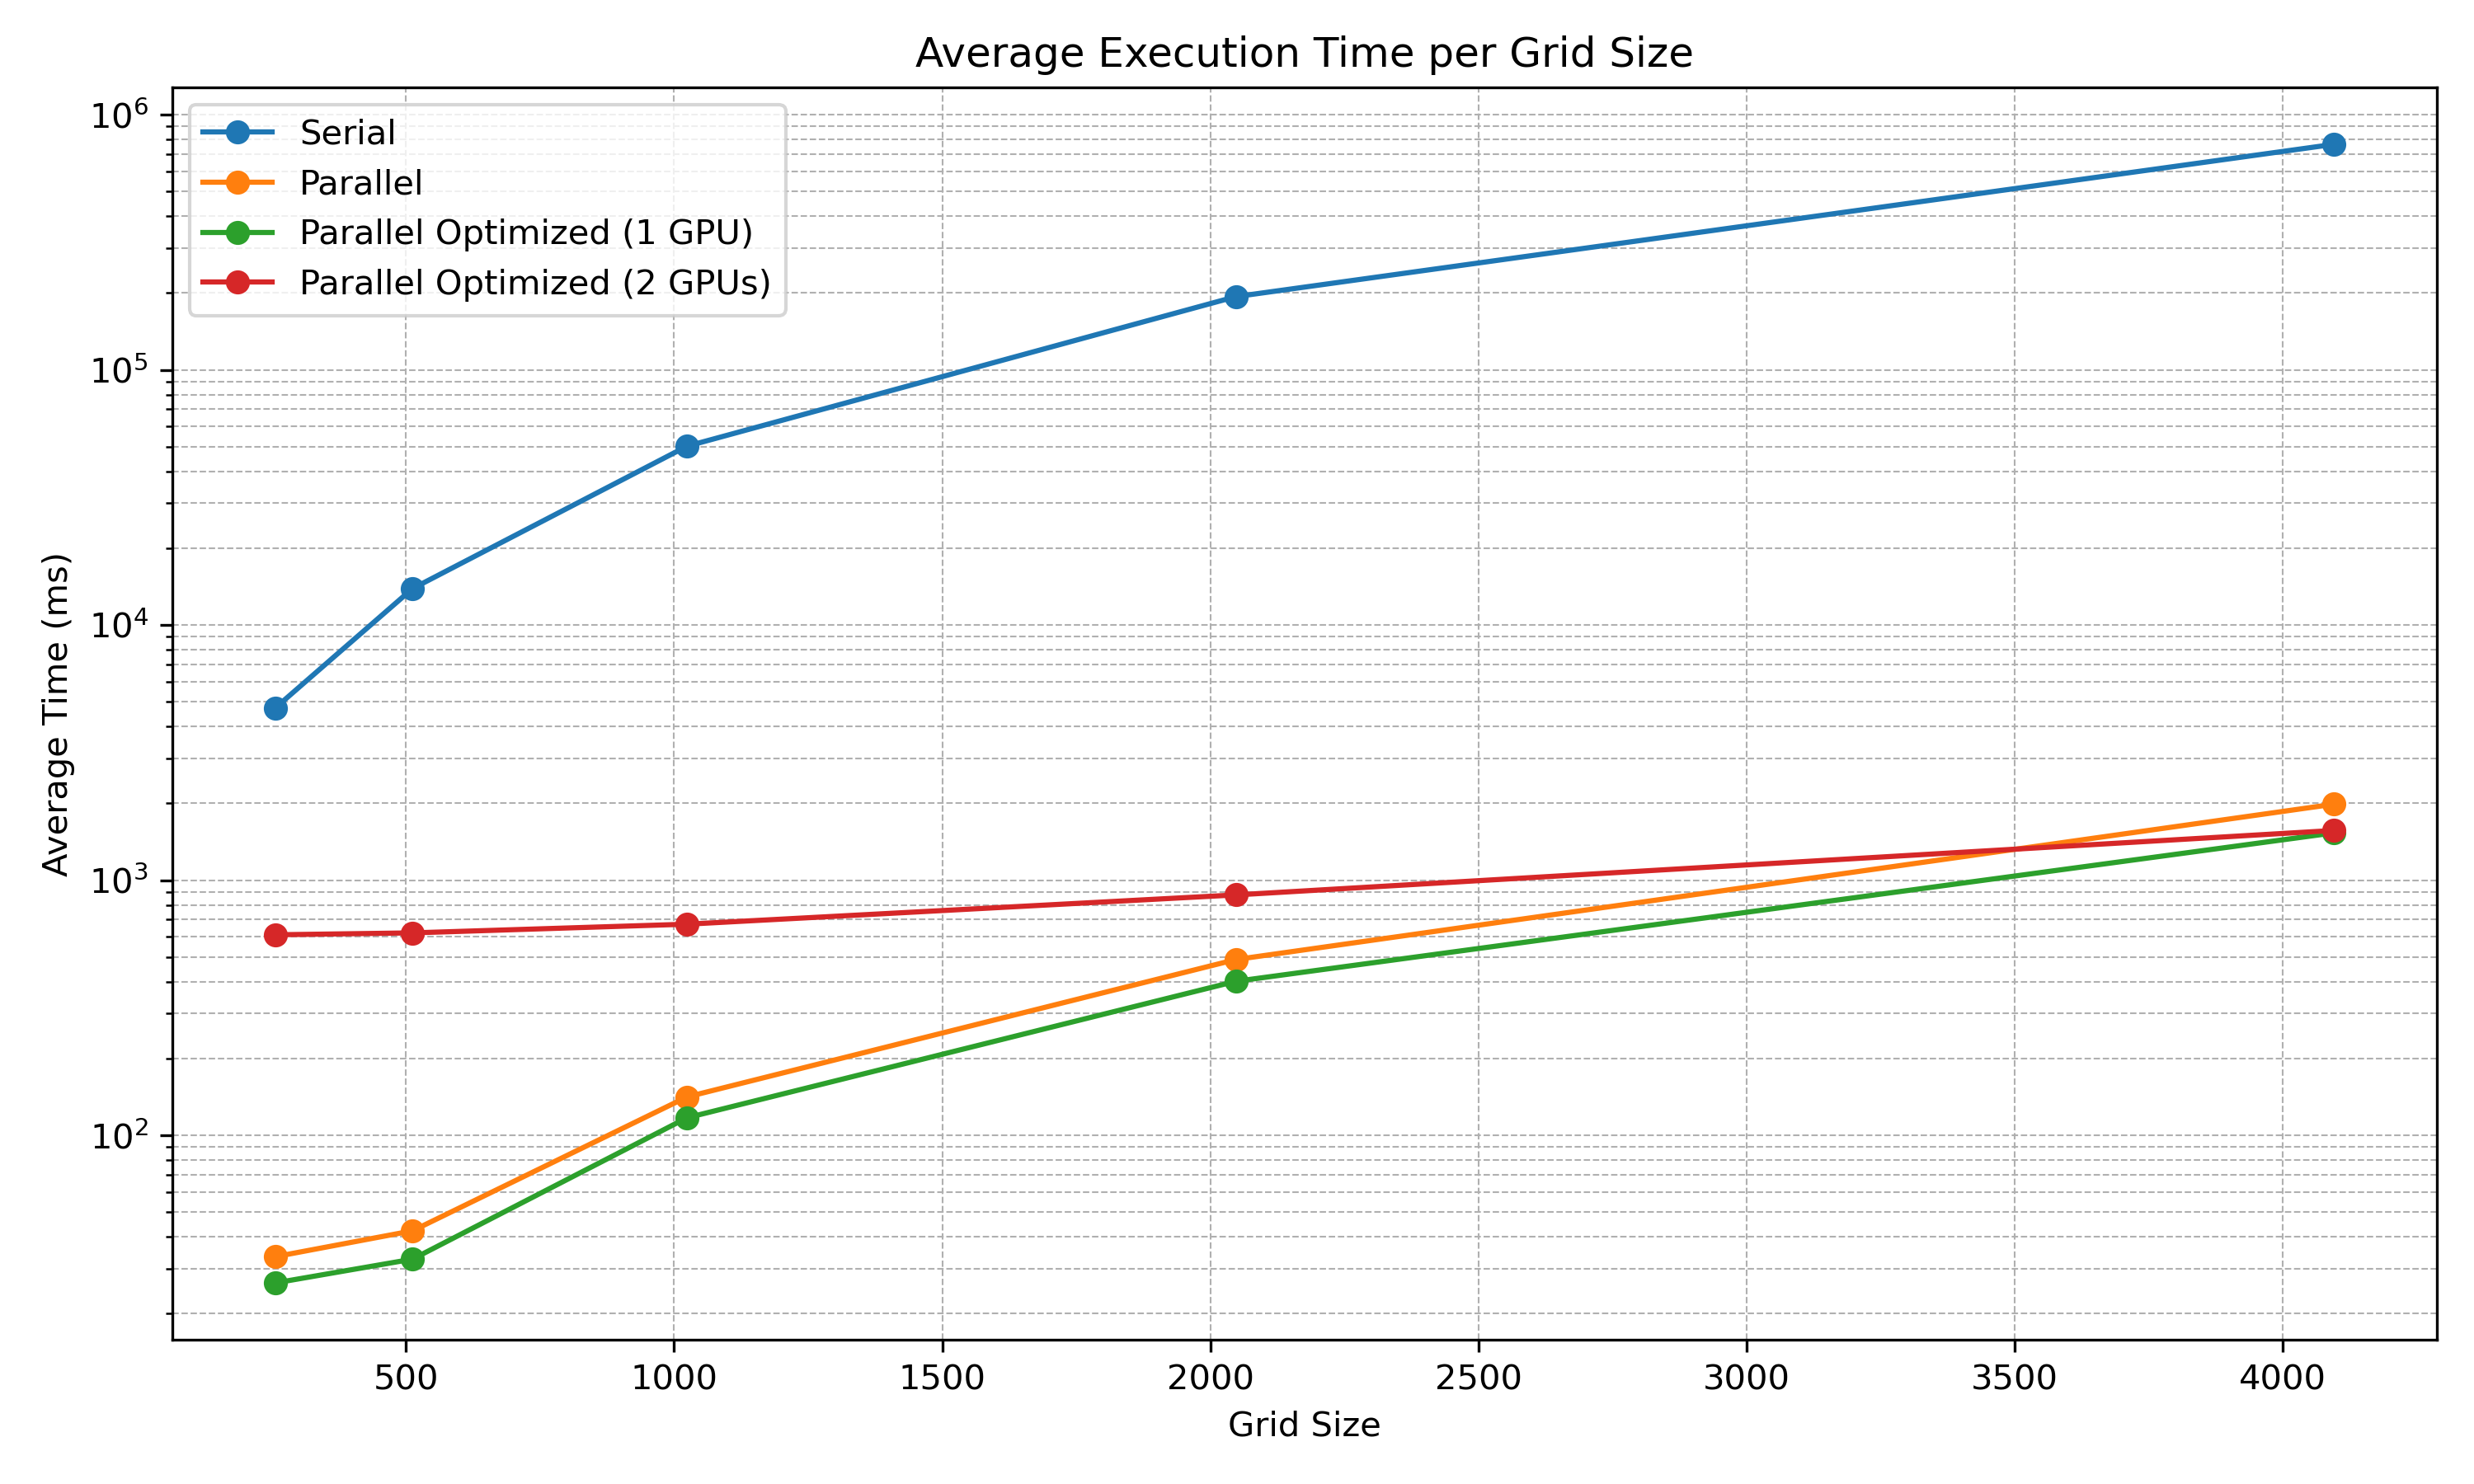
\includegraphics[width=1.0\linewidth]{img/execution_time_comparison.png}
    \caption{Average execution time measured in \textbf{milliseconds [ms] in log scale} of each algorithm for each grid size, shown in Table~\ref{tbl:avg_times}.}
    \label{fig:avg_times}
\end{figure}


\begin{table}[H]
    \centering
    \begin{tabular}{| l || c | c | c | c | c |}
        \hline
        Comparison with serial & 256x256 & 512x512 & 1024x1024 & 2048x2048 & 4096x4096 \\
        \hline
        Parallel & 141 & 329 & 355 & 396 & 386 \\
        Parallel Optimized (1 GPU) & 179 & 425 & 428 & 482 & 500 \\
        Parallel Optimized (2 GPUs) & 8 & 22 & 75 & 221 & 489 \\
        \hline
    \end{tabular}
    \caption{Average speedup calculated between execution times for each grid size.}
    \label{tbl:speedups}
\end{table}

\begin{figure}[H]
    \centering
    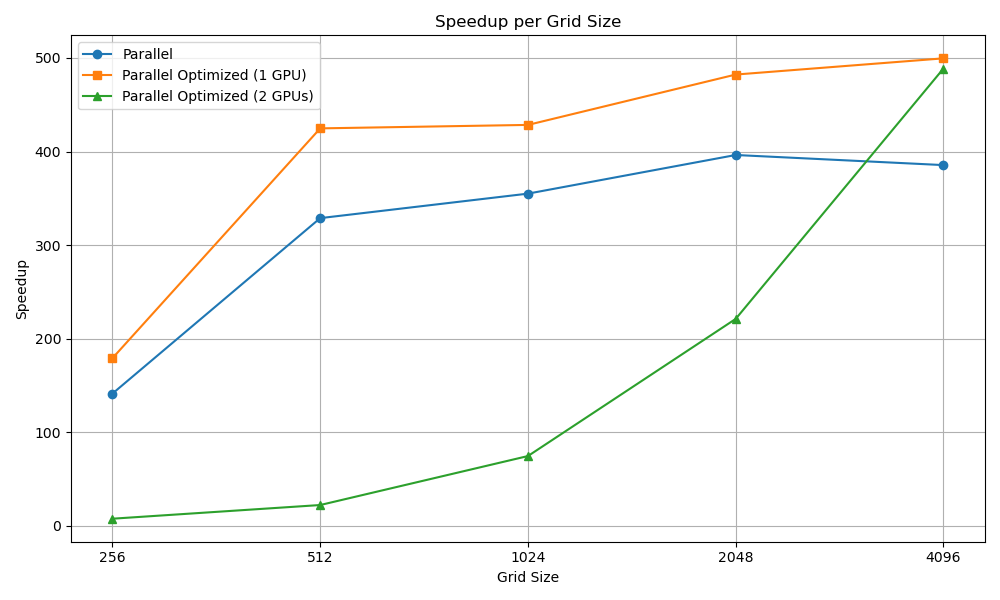
\includegraphics[width=1.0\linewidth]{img/speedup.png}
    \caption{Average speedup calculated between execution times for each grid size, shown in Table~\ref{tbl:speedups}.}
    \label{fig:speedups}
\end{figure}

We also tried different shapes of blocks of threads (in parallel algorithm) and observed a small 5\% improvement with the stripe shape compared to the block shape.

\end{document}
